\documentclass[12pt,letterpaper]{article}


\usepackage{hyperref}
\usepackage{amsmath}
\usepackage{listings}
\usepackage{graphicx}


\begin{document}
\title{Evac Sim: Fall 2020 CSS600 }

\author{Justin Downes and Chris Smith}
\date{December 2020}
\maketitle

\begin{abstract}
Simulating large scale evacuation is cost-prohibitive in terms of realism and
required man-hours. Agent-based simulation supports laying out a floorplan,
modeling behaviors and at least capturing some flavor of how a real evacuation
might play out. This research uses NetLogo to vary floorplans and capture the
average escape times for the agents.
\end{abstract}
\section {Introduction}
\section {Background}
\subsection{Previous Work}
The literature abounds with previous efforts in this area.
\cite{almeidaCrowdSimulationModeling2013} 
\cite{kneidl}
\cite{kuligowskil}
\cite{abmEvac}
\cite{zhouSimulationPedestrianEvacuation2019}

This paper is key as it is extremely similar and a NetLogo implementation.  We should know this paper and incorporate into our paper \cite{prioritEvac}

\section {Methodology}
The simulation itself is straightforward, and makes novel use of the Behavior
Space facility, which we wrapped in a Python driver making use of pytest which
is laid out in scripts/tests/test_fire_sim.py
\subsection{Environment}
For the map files in use, there were 10 runs against the map files, capturing
mean-escape-time for the agents.
\begin{figure}
  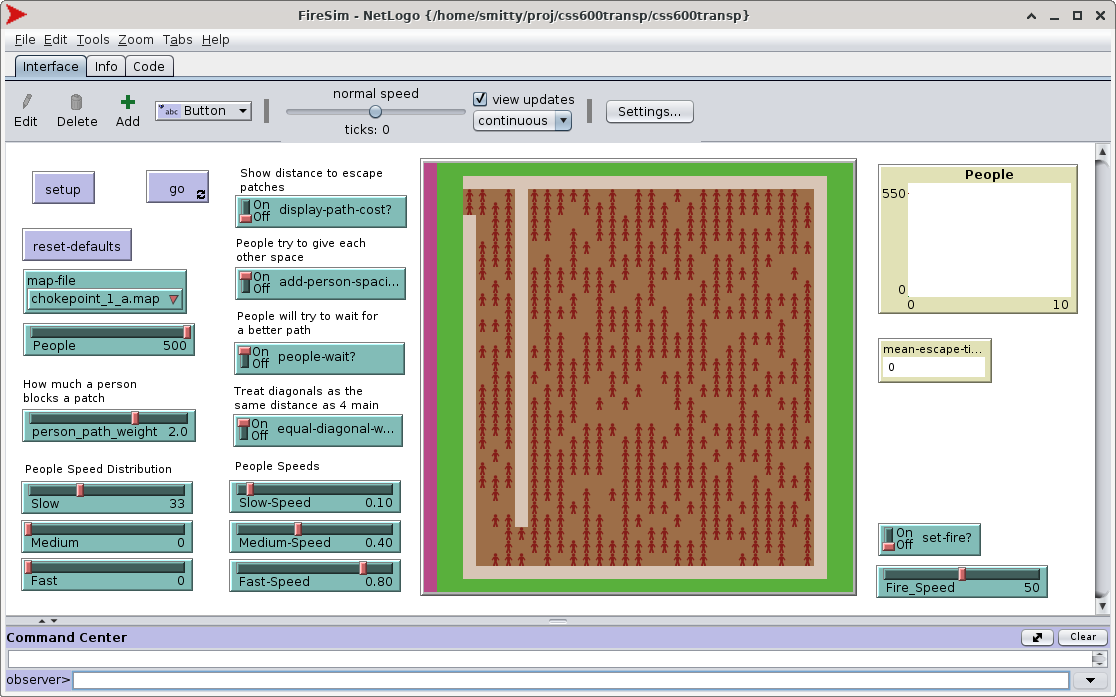
\includegraphics[width=\linewidth]{./figures/fire_sim_ui.png}
  \caption{FireSim UI}
\end{figure}

\begin{tabular}{ l | l }
map-file & Name of map file to set up. \\
People & Number  of people. Held constant at 500. \\
person_path_weight & Agent blockage factor for patch \\
Slow & Percentage moving at this rate, which we set to 100 \\
Medium & Set to 0 \\
Fast & Set to 0 \\
Slow-Speed & 0.3 patches \\
Medium-Speed & 0.75 patches \\
Fast-Speed & 1.0 patches \\
add-person-spacing? & true \\
equal-diagonal-weight? & true \\
display-path-cost? & false \\
people-wait? & true \\
set-fire? & false \\
Fire_Speed & 50 \\
mean-escape-time & output \\
\end{tabular}

need to talk about patch parameters
\subsection{Movement Mechanisms}
this section will discuss agent and fire movement algorithms

The cost algorithm, where $P_s$ is a safety patch, where $A_w$ is the person path weight, a weight that a person adds to a patch due to blocking (this is configurable by the user)
\begin{align}
cost(P)  = distance(P_s, P) + Agent(P) * A_w \nonumber \\
Agent(P)=
\begin{cases}
1, & \text{Agent Present}  \\
0, & \text{Agent Not Present} 
\end{cases}
\end{align}

this can be configured through equal diagonal weight flag. if False the Distance is the Manhattan distance \footnote{ https://www.sciencedirect.com/topics/mathematics/manhattan-distance}. If true the distance is the Chebyshev Distance \footnote{https://en.wikipedia.org/wiki/Chebyshev\_distance}
\begin{align}
distance(P_1, P_2)  = \nonumber\\
equal-diagonal-weight?=
\begin{cases}
	max(|x_1-x_2|, |y_1-y_2|), & True \\
	|x_1-x_2|+ |y_1-y_2|, & False
\end{cases}
\end{align}


patch to move to algorithm, where $A_p$ is the patch for a given agent, $P_x$ \& $P_y$ are the $X$ \& $Y$ coordinates for a given patch
\begin{align}
neighbors_4 (P)  = \{patch(P_x - 1, P_y -1), patch(P_x + 1, P_y -1), \nonumber \\ 
patch(P_x - 1, P_y + 1),patch(P_x + 1, P_y + 1)\}   
\end{align}

\begin{equation}
move(A) = min(cost(neighbors_4 (A_p)))
\end{equation}

Person will wait for a better patch.  This is configurable by the user. If it is on then a person will wait for a patch that is less cost than it's current
\begin{equation}
people-wait?=
\begin{cases}
min(cost(A_p), move(A)), & True\\
move(A), & False
\end{cases}
\end{equation}

add person spacing algorithm, people try to avoid each other, configurable through the $add-person-spacing?$ flag and the $person\_path\_weight$, $A_w$, parameter.  here, $A_w$, is scaled by a factor of 10 since it is not the weight of being in the same square as another but of being next to another person.

\begin{equation}
add-person-spacing?=
\begin{cases}
	cost(P) \sum Agent(neighbors_4(P)) * A_w / 10, & True \\
	cost(P), & False
\end{cases}
\end{equation}

\cite{mirahmadiNovelAlgorithmRealtime2012}
\footnote{http://www.cs.us.es/~fsancho/?e=131}

\subsection{Experiments}

describe our experiment harness that we built, netlogo behavior space, sql alchemy

\subsubsection{experiments that are based on layouts.}  

-exit dims maps:  see if placement has an effect on mean and max escape time.  line plot for each number connecting a,b, and c points where each point is the average of multiple (10) runs . separate plots for mean and max

- choke point escape: same as above

- need to run experiment on using a.map that plots mean escape time as we increase number of agents.  probably 50 to 500 step size 10. we would expect to see this scale linearly but if not then there may be an interesting story.

\subsubsection{experiments that are based on agent mechanisms}

- vary experiments of person path weighting and agent speeds/distributions

\subsubsection{experiments that are based on patch parameters.}

-  this may be obe by the exclusion of the fire mechanism

\subsubsection{experiments that replicate emergent crowd behaviors from other papers}
- maiinly from this paper \cite{almeidaCrowdSimulationModeling2013}  .  

- herding and flocking

-arching and crowding

if we can show that we achieve similar results even though we use a simplified pathing algorithm and abm environment i think that would be insightful


\section{Results}



\section {Conclusion}

\bibliographystyle{plain}
\bibliography{css600}

\end{document}
